\begin{figure}
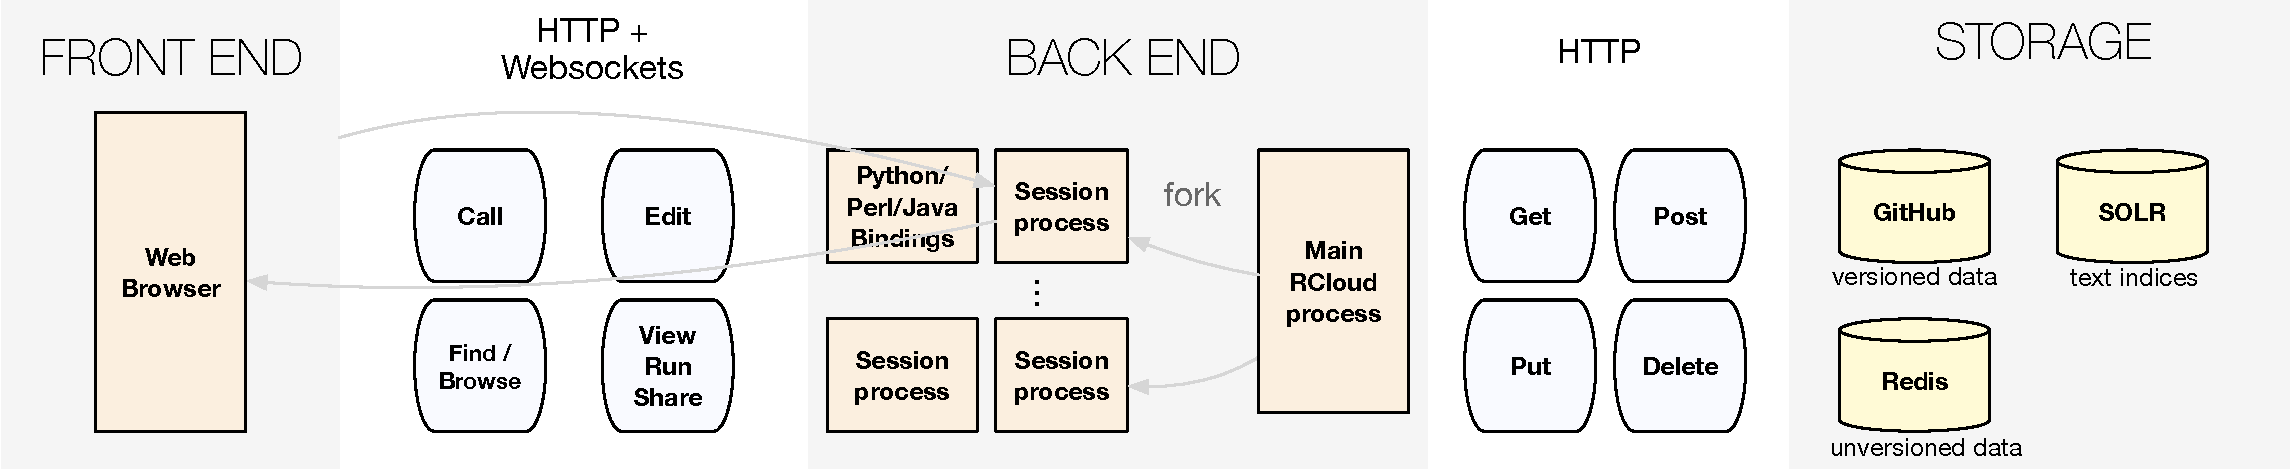
\includegraphics[width=\linewidth]{fig/system/system.pdf}
\caption{\label{fig:system}A diagram of RCloud's architecture. Dashed
  lines represent features which not yet implemented. \carlos{Must remove anything that isn't implemented}}
\end{figure}

\section{Related Work}

\carlos{There's no need to position ourselves defensively here; we're
  addressing different needs, and the connection is already
  tenuous. We're just hurting ourselves by comparing to wrangling and
  then saying ``well, we don't have wrangling''}

Kandel et al. argue in their review of data wrangling work that data
cleaning, wrangling and transformation is a major part of exploratory
analysis and visualization~\cite{Kandel:2011:RDI}. Although RCloud
does not by itself include modules specific to data cleaning and
wrangling, we note from practical experience that these cleaning
scripts themselves tend to change over time. RCloud addresses this
issue by providing easy publishing of data-cleaning notebooks as web
services, which reduces the total data-cleaning effort across an
organization.

Kandel et al.'s interview study points out the typical ``explore'',
``model'', ``report'' cycle in enterprise data
analysis~\cite{Kandel:2012:EDA}. There are many discontinuities in
this cycle that cost time and effort to overcome. RCloud seeks to
reduce this mismatch. They also point out that larger teams
are becoming more common in data analysis, that supporting
collaboration is a difficult and important problem, and that sharing
and versioning of data sources and artifacts is hindered by current
technology in practice. ``We found that analysts typically did not
share scripts with each other. Scripts that were shared were
disseminated similarly to intermediate data: either through shared
drives or email. Analysts rarely stored their analytic code in source
control.'' Their work points to the opportunity for better technology
to support collaboration and sharing by data analysis teams.

Heer and Agarwala identify many design considerations for
collaborative visual analytics~\cite{Heer:2008:DCF}.
Notebooks, and the integrated version control system for them, described in
Section~\ref{sec:notebooks}, address modularity and granularity, and
artifact histories.
\emph{Starring}, the means for signaling interest in notebooks, described in
Section~\ref{sec:starring}, addresses social-psychological incentives,
recommendation, and voting and ranking. RCloud's integrated deployment
mechanism, described in Section~\ref{sec:deployment}, addresses cost of
integration, content export, presentation and view sharing.

Manyeyes \cite{Viegas:2007:MAS} was a landmark system for the integration
of social media with visualization and data publishing. We build on this
work by defining a rich interface for collaboration about code and for
operating on metadata.

The need for integrating statistics and visualization has been
highlighted in previous studies and is widely understood by
various technical communities \cite{Perer:2008:ISA}
Lucas and Roth were early advocates of combining
data exploration with presentation and publication \cite{Lucas:1996:EIV}.

There has been noteworthy work on specific techniques such as
social bookmarking \cite{Millen:2006:DSB} \cite{Heer:2007:VAV}
and crowdsourcing \cite{Fast:2014:ECS} to support collaborative
or social development or analysis processes.
Similarly, there are computational methods to support high
performance execution in incremental code development
environments \cite{Guo:2010:TPI}.
Our goal is to define an environment in which many such
techniques may be integrated and made available to a broad community.

VisMashup~\cite{Santos:2009:VST} and Crowdlabs~\cite{Mates:2011:CSA}
are tools built on top of the VisTrails workflow management
system~\cite{Callahan:2006:VVM}. VisMashup defines a schema and
semantics for automatically deriving user interfaces from workflows,
while Crowdlabs exposes these capabilities on a website feature
workflow upload and remote execution. In our view, the impedance
mismatch between a dataflow pipeline specification and the power of a
general-purpose language is too great for the type of general
exploratory work in data science teams. As a result, RCloud tries to
provide a closer match for analysts accustomed to creating and
executing R and Python code, while retaining many attractive
properties like automatic versioning and management.

\begin{figure*}
\centering
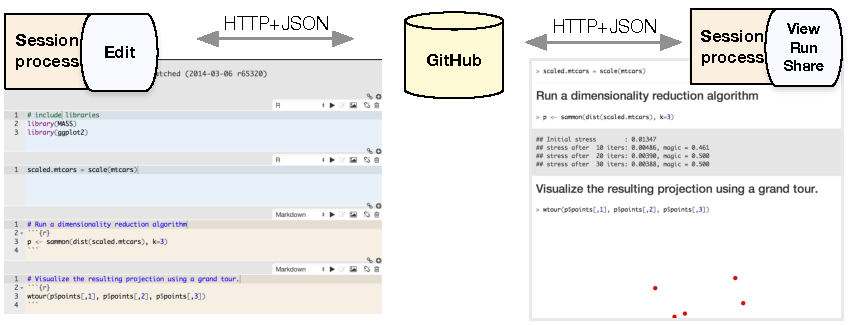
\includegraphics[width=.8\linewidth]{fig/notebook/notebook.pdf}
\caption{\label{fig:notebook}An RCloud notebook is a sequence of
  \emph{cells}, each a snippet of source in R or Markdown. Notebooks
  are stored in GitHub \emph{gists}, which provide the version-control
  primitives needed in RCloud during editing (left) or viewing and
  executing (right).}
\end{figure*}

Our work has been inspired by and benefited from other efforts
to improve data analysis environments and processes,
including RStudio \cite{RStudio:2013:SWA},
the R packages Markdown \cite{Allaire:2014:MMR},
knitr \cite{Xie:2013:DDW}
and Shiny \cite{RStudio:2013:SWA},
and iPython notebooks \cite{Perez:2007:IAS}
to name a few. RStudio aims at providing an integrated development environment
for R, with support for publishing code in packages. Markdown,
knitR and Shiny provide R with sophisticated reporting capabilities, including
interactive web interfaces. IPython \cite{Perez:2007:IAS}
shares many of our goals, such as providing a comprehensive environment
for analysis and programming, and shareable documents on the web.

One overall goal is to reduce the gap between implementers and deployers
of technology in visual analytics. The fusion of development with production
operations in software release management (``DevOps'' \cite{Httermann:2012:DD})
is a trend in web services and related fields. By making it possible
for data scientists to expend a little more effort in the process of
creating experiments, it may be possible to eliminate the need for
programming teams to recreate their results in production with
a concomitant penalty in time and expense.
